\section{Other design decisions}
\subsubsection{Subdivision into components}
\paragraph{}From the previous sections is clear that all our architectural design is highly oriented to the subdivision of the entire system into submodules, having each of them a different role in the achieving of the requirements of our application. We can call this approach \textit{component-oriented}.\\
It is basically an application of the \textit{divide and conquer} design principle.

\subsubsection{Dependency inversion principle}
\paragraph{} We have taken care of always provide interfaces for the subcomponents applying so the \textit{dependency inversion principle}. The various components of the system depend only on the interfaces of the others and never on the internal representation.

\subsubsection{Deployment choices}
\paragraph{} As far as the deployment is concerned, we have already seen that our choice is to deploy both the business logic (application server) and the web management (web server) on the same machine.\\ We must say that our RASD did not specify any constraint about deployment and so we opted for the easiest and cheaper solution for our clients.\\ A future enhancement may be to delegate the data logic to a clouding infrastructure with a remote server. This possible choice will bring the following advantages:
\begin{itemize}
	\item \textit{Division of responsibility}: the data storage is delegated to a specialize provider which can manage it with advanced control systems. This feature brings to the following advantages.
	\item \textit{Security}: to have the data stored far away from the Main Server enhance security
	\item \textit{Easy scalability} of the database 
\end{itemize}

\subsubsection{Programmatic interface} \label{design:programmaticInterface}
\paragraph{} For the satisfiability of the requirement to have a programmatic interface that can make the developers able to build new functionalities on the top of the already provided, we decided to expose all the component interfaces that we have described (figure \ref{fig:programmaticInterface}).

\begin{figure}[H]
	\centering
	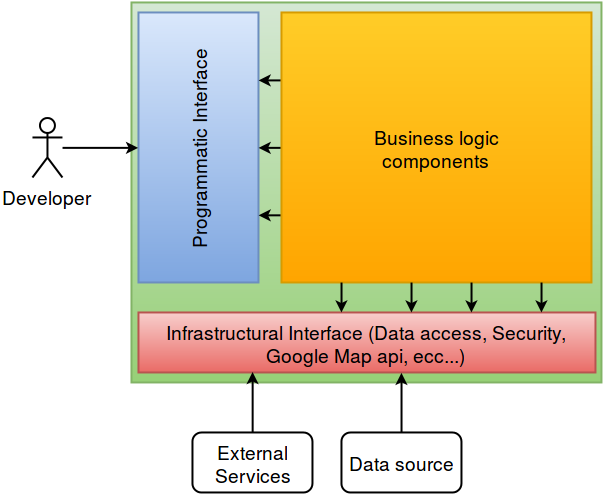
\includegraphics[scale=0.35]{../"Analysis Documents"/programmaticInterface}
	\caption{Schematic representation of the role of the programmatic interface in the system}
	\label{fig:programmaticInterface}
\end{figure}
